%%%% ijcai21-multiauthor.tex
\pdfoutput=1

\typeout{IJCAI--21 Multiple authors example}

% These are the instructions for authors for IJCAI-21.

\documentclass{article}
\pdfpagewidth=8.5in
\pdfpageheight=11in
% The file ijcai21.sty is NOT the same than previous years'
\usepackage{ijcai21}

% Use the postscript times font!
\usepackage{times}
\renewcommand*\ttdefault{txtt}
\usepackage{soul}
\usepackage{url}
\usepackage[utf8]{inputenc}
\usepackage[small]{caption}
\usepackage{graphicx}
\usepackage{amsmath}
\DeclareMathOperator*{\argmax}{argmax} % thin space, limits underneath in displays
\usepackage{booktabs}
\urlstyle{same}
\usepackage{float}
\usepackage{bm}
\usepackage{amsfonts}
\usepackage[numbers]{natbib}
\usepackage[dvipsnames,table,xcdraw]{xcolor}
\usepackage{subcaption}
\usepackage{graphicx}
\usepackage{wrapfig}

% import package for multi row and graphics
\usepackage{multirow}
\usepackage{graphicx}
\usepackage{placeins}
\usepackage{booktabs,makecell,tabularx}
\usepackage{hyperref}

\setlength\parindent{0pt}
% footnote no indent
\usepackage[hang,flushmargin]{footmisc}

% the following package is optional:
%\usepackage{latexsym}

% Following comment is from ijcai97-submit.tex:
% The preparation of these files was supported by Schlumberger Palo Alto
% Research, AT\&T Bell Laboratories, and Morgan Kaufmann Publishers.
% Shirley Jowell, of Morgan Kaufmann Publishers, and Peter F.
% Patel-Schneider, of AT\&T Bell Laboratories collaborated on their
% preparation.

% These instructions can be modified and used in other conferences as long
% as credit to the authors and supporting agencies is retained, this notice
% is not changed, and further modification or reuse is not restricted.
% Neither Shirley Jowell nor Peter F. Patel-Schneider can be listed as
% contacts for providing assistance without their prior permission.

% To use for other conferences, change references to files and the
% conference appropriate and use other authors, contacts, publishers, and
% organizations.
% Also change the deadline and address for returning papers and the length and
% page charge instructions.
% Put where the files are available in the appropriate places.

%PDF Info Is REQUIRED.
\pdfinfo{
/TemplateVersion (IJCAI.2021.0)
}

\title{Apply watermarking algorithm to LLM-based text summarization model}

\author{
Xuefei Jiang
\affiliations
School of Computer Science, University College Dublin, Dublin, Ireland
\emails
sc.xfjiang@gmail.com
}

\begin{document}
\maketitle
\section{Introduction}
In this experiment, the primary focus is on two main aspects:
\begin{enumerate}
	\item The development of an abstractive summarization model based on the T5 architecture \cite{raffel2020exploring}.
	\item The application of the watermarking algorithm as described by \cite{kirchenbauer2023watermark}, with a subsequent discussion on its effects on the performance of the original summarization model.
\end{enumerate}

\section{Method}
The abstractive summarization task inherently aligns with the sequence-to-sequence paradigm, making the encoder-decoder LLM a natural selection. Consequently, the T5 model is chosen. Different variants of the T5 model, along with their corresponding numbers of parameters, are depicted in Table \ref{tab:t5}.

\begin{table}[H]
	\centering
	\begin{tabular}{|c|c|}
		\hline
		model & \#parameters \\ \hline
		Tiny  & 16M          \\ \hline
		Mini  & 31M          \\ \hline
		Small & 60M          \\ \hline
		Base  & 220M         \\ \hline
		Large & 738M         \\ \hline
		3B    & 3B           \\ \hline
		11B   & 11B          \\ \hline
	\end{tabular}
	\caption{Different versions of the T5 model}
	\label{tab:t5}
\end{table}

I have two A100 (40G) GPUs without NVLink or PCIE connection. I aimed to employ the largest feasible models to harness the full capabilities of my GPUs. The suitable hyperparameters for this experiment and the corresponding GPU memory usage are outlined in Table \ref{tab:gpu_memory}, which closely approaches the limit of my devices.
\begin{table}[H]
	\centering
	\begin{tabular}{|c|c|c|}
		\hline
		model & batch size & \#parameters \\ \hline
		T5 Base  & 32         & 39507MB     \\ \hline
		T5 Large & 8          & 35357MB     \\ \hline
	\end{tabular}
	\caption{GPU memory usage}
	\label{tab:gpu_memory}
\end{table}

The developed code successfully works on both datasets:
\begin{itemize}
	\item \href{https://www.kaggle.com/datasets/gowrishankarp/newspaper-text-summarization-cnn-dailymail}{CNN-DailyMail News Dataset}
	\item \href{https://www.kaggle.com/datasets/sunnysai12345/news-summary}{News Summary Dataset}
\end{itemize}

The core statistics of the two datasets are illustrated in Table \ref{tab:dataset_stat}.

\begin{table}[H]
	\begin{tabular}{|c|c|c|}
		\hline
		model              & CNN-DailyMail News & News Summary \\ \hline
		\# train instances & 287113            & 3611         \\ \hline
		\# test instances  & 11490             & 903          \\ \hline
	\end{tabular}
	\caption{Dataset statistics}
	\label{tab:dataset_stat}
\end{table}

However, I have found that conducting experiments on the CNN-DailyMail News Dataset is significantly more time-consuming compared to the News Summary Dataset, especially when using the T5-large model. At the time of writing this report, the experiments on the CNN-DailyMail News Dataset are still in progress. Therefore, for the purpose of this report, I will only present and discuss the results obtained from experiments that are already finished. \\

The watermarking algorithm has been incorporated into the T5-based summarization model, serving as a LogitsProcessor to adjust the output probabilities of the language model. Core Python files from the repository \href{https://github.com/jwkirchenbauer/lm-watermarking}{A Watermark for Large Language Models} were included in my repo as modules to apply the watermarking algorithm.

\section{Results}
Table \ref{tab:rouge-scores_news} and \ref{tab:rouge-scores_cnn} illustrates how watermarking affects the performance of the summarization model. As the results indicate, the application of watermarking unsurprisingly lowers the performance. This reduction in effectiveness is attributable to the watermarking algorithm's adjustment of the output probabilities of the language model. By doing so, it constrains the choices available to the language model, thus negatively impacting its performance.\\

In addition to watermarking, an investigation into how model size influences summarization performance was conducted. The findings reveal that a larger model size enhances the performance of the summarization.\\

\begin{table*}[h]
	\centering
	\begin{tabular}{lccc}
		\hline
		& ROUGE-1 & ROUGE-2 & ROUGE-L \\
		\hline
		T5-base without watermarking  &  0.4832 &  0.2642 &  0.3631 \\
		T5-base with watermarking     &  0.4616 &  0.2321 &  0.3345 \\
		T5-large without watermarking &  \textbf{0.4901} &  \textbf{0.2697} &  \textbf{0.3632} \\
		T5-large with watermarking    &  0.4780 &  0.2401 &  0.3413 \\
		\hline
	\end{tabular}
	\caption{Comparison of ROUGE scores for different models on News Summary Dataset}
	\label{tab:rouge-scores_news}
\end{table*}

\begin{table*}[h]
	\centering
	\begin{tabular}{lccc}
		\hline
		& ROUGE-1 & ROUGE-2 & ROUGE-L \\
		\hline
		T5-base without watermarking  &  still training &  still training &  still training \\
		T5-base with watermarking     &  still training &  still training &  still training \\
		T5-large without watermarking &  still training &  still training &  still training \\
		T5-large with watermarking    &  still training &  still training &  still training \\
		\hline
	\end{tabular}
	\caption{Comparison of ROUGE scores for different models on CNN-DailyMail News Dataset}
	\label{tab:rouge-scores_cnn}
\end{table*}

However, although the results presented above are consistent with expectations, there are some aspects that remain perplexing. For instance, in all experiments, the training converges very early, as illustrated in Figure \ref{fig:trainloss}, indicating that the model does not extract as much information from the substantial volume of data as anticipated.

\begin{figure}[H]
	\centering
	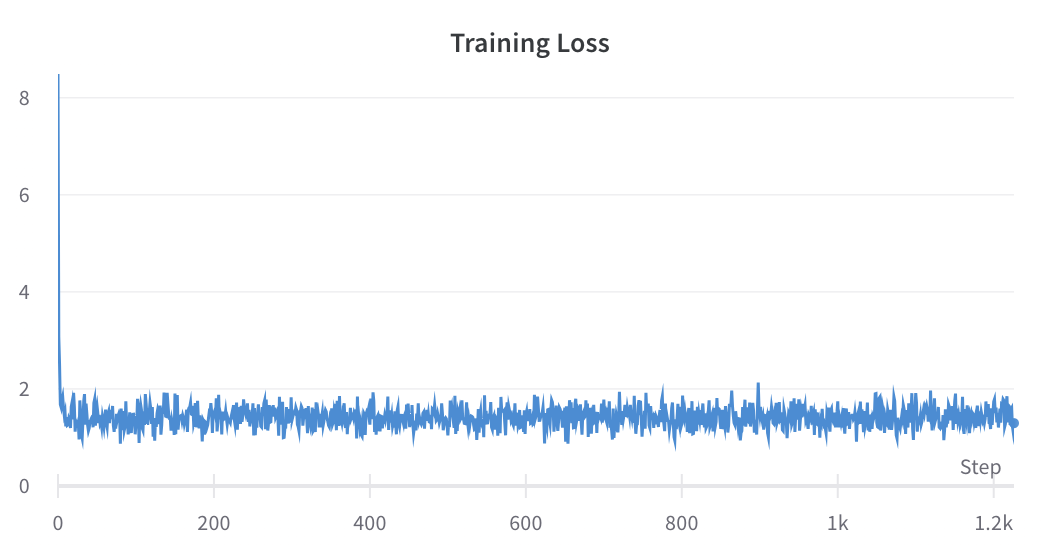
\includegraphics[width=1.0\linewidth]{images/train_loss}
	\caption{train loss}
	\label{fig:trainloss}
\end{figure}

I believe the main cause of this phenomenon is that the T5 model already has strong summarization capabilities and doesn't require a lot of data to be tuned. The ability of summarization cannot be increased by adding more training data unless new strategies are added to it.

\appendix
\section*{Appendix: Watermark Algorithm}
Warkmarking is the process of embedding signals into generated text that are invisible to humans but can be identified algorithmically by watermark detection algorithms.  In this section, I will discuss the algorithms provided in \cite{kirchenbauer2023watermark}.

\begin{figure}[H]
	\centering
	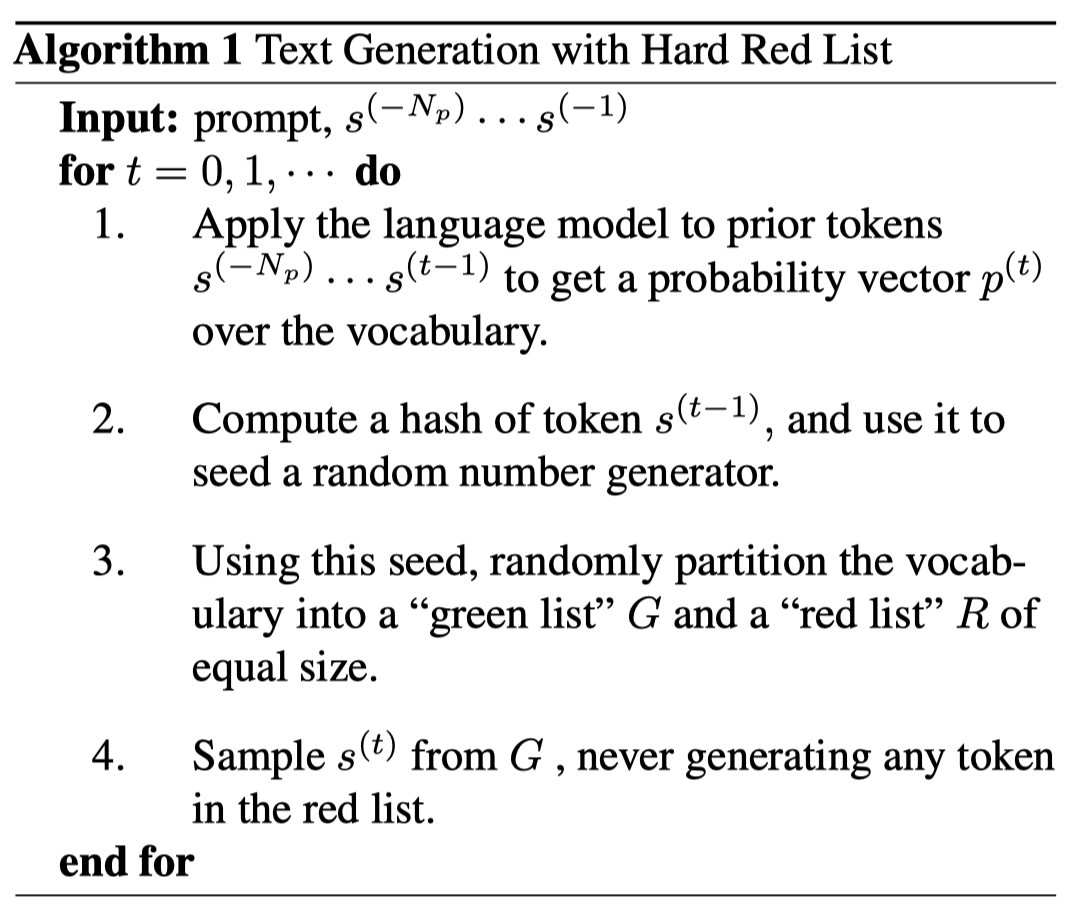
\includegraphics[width=1.0\linewidth]{images/watermark_1}
	\caption{Algorithm 1}
	\label{fig:watermark1}
\end{figure}
In Algorithm 1, given the prompt $ s^{(-N_p)}\dots, s^{(-1)} $, a probabilistic language model is employed to predict the subsequent word in a sequential manner. However, at each time step, the probability of a certain group of words (termed as RED LIST) is manually set to zero, ensuring they never appear at that specific time step. Conversely, only a select portion of the vocabulary (referred to as the GREEN LIST) is allowed to appear. This approach essentially embeds statistical features within the model, which can subsequently be identified by a detection algorithm. \\

The detection of watermarks operates entirely within the framework of statistical hypothesis testing, largely due to the fact that we're adjusting the probability distribution of words at each timestep. For a text sequence of the same length $N$, a natural language generator would breach the GREEN/RED LIST rule with a probability of $ 50\% $, while a watermarked text generator would not. Consequently, the expected number of words that break the GREEN/RED LIST rule should be $N/2$. We can then establish a one-sample $z$-test to test this expected value (with variance unknown). The testing statistic is as follows:

\begin{equation}\label{key}
	T(x) = \dfrac{\sqrt{n}\left(\bar{X} - \mu_0\right)}{S}
\end{equation}

where
\begin{itemize}
	\item $ n = N $
	\item $\bar{X}$ is the number of words that breach the GREEN/RED LIST rule.
	\item $\mu_0 = N/2$
	\item $S$ is the sample variance (however, in the original paper, $S$ is set to the expected variance $N/4$).
\end{itemize}

Then, we can use this statistic to test if the text sequence is generated by a watermarked text generator. Certainly, we can change the proportion $ 50\% $ to another value to give the text generator more options to improve the quality of the generated text.

\begin{figure}[H]
	\centering
	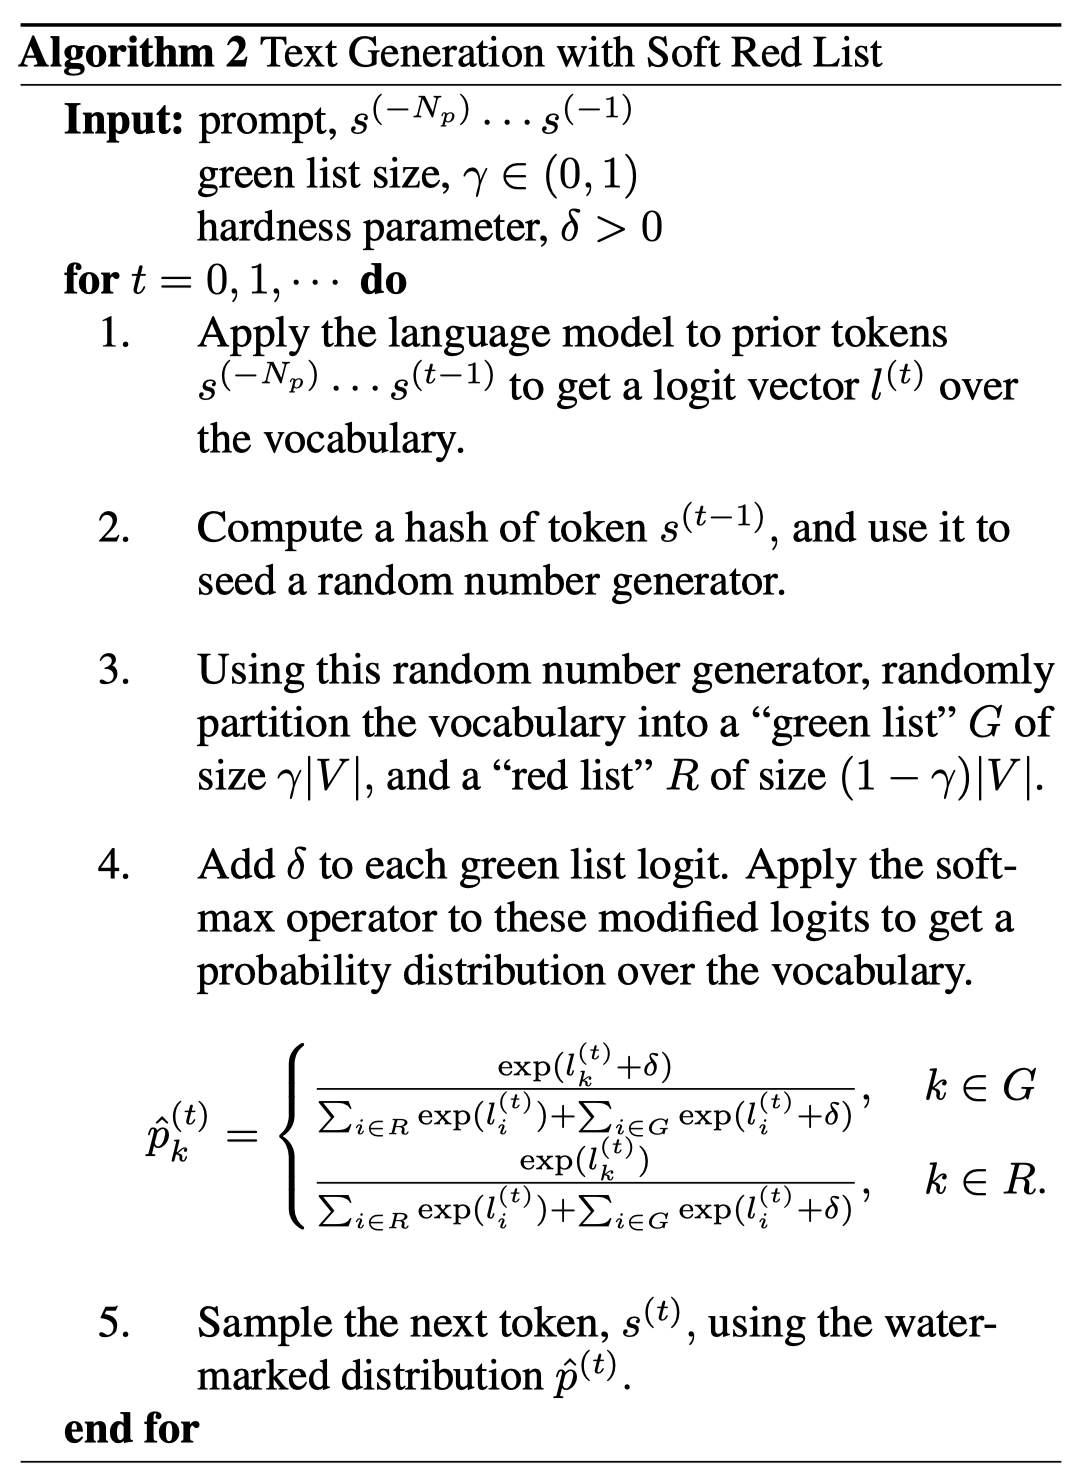
\includegraphics[width=1.0\linewidth]{images/watermark_2}
	\caption{Algorithm 2}
	\label{fig:watermark2}
\end{figure}
Algorithm 2 is a more advanced version of Algorithm 1, but the methodology remains unchanged. Instead of simply setting all probabilities of words in the RED LIST to zero, Algorithm 2 increases the probability of words in the GREEN LIST. Such manipulation of the probability distribution still allows for the detection algorithm to identify watermarked texts.\\

When I first read this paper, I was more interested in the detection of watermark. However, I noticed that the detection algorithm relies heavily on familiarity with the watermarking algorithm's specifics - for instance, the hashing function utilized to create the RED/GREEN list. This concept doesn't quite sit right with me, given it implies the need for additional information for the detection algorithm to function effectively. I am optimistic that future developments will bring forth a detection algorithm capable of discerning whether a text has been machine-generated, without the need to comprehend the intricacies of the watermarking algorithm. In my view, this back-and-forth dynamic of text generation and detection will persist until we arrive at true AGI. Just brainstorming.

%----------------------------------------------------------------------------------------
%	BIBLIOGRAPHY
%----------------------------------------------------------------------------------------
\bibliographystyle{abbrv}
\bibliography{reference}
\setcitestyle{citesep={,}}

\end{document}
